%!TEX root = ../dokumentation.tex
\chapter{Backend}\label{ch:backend}
Als Backend wurde eine REST-API mit Node.js und dem Webframework Express entwickelt.

\section{Struktur}
Der Startpunkt des Backends ist die \hyperlink{https://github.com/Drinkler/Online-Shop/blob/master/backend/app.js}{app.js} Datei im Backend Ordner. Dort werden Daten initialisiert, Einstellungen vorgenommen, der Server mit der Datenbank verbunden und auch der Server gestartet.\\
Die eigentliche Struktur befindet sich im \hyperlink{https://github.com/Drinkler/Online-Shop/blob/master/backend/api}{api Ordner}. In diesem befindet sich eine \hyperlink{https://github.com/Drinkler/Online-Shop/blob/master/backend/api/index.js}{index.js} Datei. Diese Datei definiert alle Basisrouten für die API.\\
Die API ist in Controller, Middlewares, Models und Routes eingeteilt.
Im Ordner Routes findet man zu jedem Model eine passende Datei. In diesen Dateien sind die dazugehörigen Routen.

\begin{lstlisting}[caption={Route von Create review (backend > api > routes > reviews.js)},label={lst:route}]
// Create review
router.post("/:userId", checkAuth, reviewValidation, ReviewController.createReview);
\end{lstlisting}

In dem Listing \ref{lst:route} ist eine Post Methode zu sehen mit dem Pfad /rest/api/reviews/:userId. Da wir bereits die reviews.js mit dem vordefiniertem Pfad aufrufen, wird nur noch der eigene Teil gebraucht. :userId ist eine Variable, die durch ein Doppelpunkt makiert ist. Danach kommen zwei Middlewares. Einmal checkAuth die prüft ob der Benutzer authorisiert ist und reviewValidation, die schaut ob der Inhalt vom Request auch korrekt ist. Zu guter letzt wird im zugehörigen Controller die createReview Funktion aufgerufen.\\
In dem Controller Ordner liegen ebenfalls für jedes Model eine Datei. In diesen Dateien ist die hauptsächtliche Logik und Verarbeitung der Daten.\\
Middlewares sind eigene unabhängige Funktionen und Aufgaben die in einer Route aufgerufen werden, z.B. das hochladen eines Bildes oder der Authorizierung.\\
In Models sind die unterschiedlichen Schemas für Mongoose, eine Wrapper für die MongoDB zur einfachen Verwaltung und Kommunikation mit der Datenbank, untergebracht.

\section{Validierung}
Zur Validierung der Request Bodies wurde das Modul \hyperlink{https://hapi.dev/module/joi/}{joi} verwendet. Es erleichtert die Validierung von Benuterdaten mithilfe einer simplen, intuitiven und einer lesbaren Sprache.

\begin{lstlisting}[caption={Validierung des Sign ups (backend > api > middleware > validation.js)},label={lst:validierung}]
const Joi = require("@hapi/joi");

const signUpValidation = (req, res, next) => {
    const signUpSchema = Joi.object({
        email: Joi.string().min(5).max(100).required().email(),
        name: Joi.string().alphanum().min(1).max(50).required(),
        surname: Joi.string().alphanum().min(1).max(50).required(),
        password: Joi.string().min(8).max(72).required(),
    });

    const { error } = signUpSchema.validate(req.body);
    if (error) return res.status(400).json({ error: error.details[0].message });

    next();
};
\end{lstlisting}

Das Listing \ref{lst:validierung} zeigt die Validierung des Sign up Requests. Die Validierung wird als Middleware in die Route eingebunden. Dadurch kann man sehr leicht sehen welche Routen eine Validierung verwenden und die Validierungen können mehrmals verwendet werden.

\section{Authorisierung}
Für die Authorizierung von Requests wurde der \hyperlink{https://jwt.io/}{JSON Web Token (jwt)} verwendet. Mithilfe dieses Tokens kann eine sichere Verbindung zwischen zwei Parteien entstehen.\\
Beim Login eines Benuters wird ein Token erstellt. 

\begin{lstlisting}[caption={Erstellung des Tokens (backend > api > controllers > user.js)},label={lst:token}]
// Create jwt token
const token = jwt.sign(
	{
		userId: user._id,
		email: user.email,
	},
	process.env.JWT_KEY,
	{
	expiresIn: "30 days",
	}
);
\end{lstlisting}

Die userId und email werden von dem Benutzer gespeichert, da man später die Daten aus dem Token lesen kann und somit abfragen kann ob es sich um ein Admin handelt.\\
Die Abfrage ob es sich um einen authorizierten Benutzer handelt und ob es ein Admin ist, wird als Middleware implementiert.

\begin{lstlisting}[caption={Abfrage des Tokens (backend > api > middleware > check-auth.js)},label={lst:checktoken}]
function checkToken(req, res, next) {
    // Check if token is given
    try {
        // If given, get user data
        const token = req.headers.authorization.split(" ")[1];
        const decoded = jwt.verify(token, process.env.JWT_KEY);
        req.userData = decoded;
    } catch (error) {
        return res.status(401).json({
            message: "User not authorized.",
        });
    }

    return req.userData;
}

const checkAuth = async (req, res, next) => {
    const userId = req.params.userId;

    const reqUser = checkToken(req, res, next);

    // check if admin
    try {
        var user = await User.findOne({ _id: reqUser.userId }).exec();
    } catch (err) {
        return res.status(500).json({ message: "Internal Server Error" });
    }

    // Check if user is authorized
    if (user.admin || reqUser.userId == userId) {
        next();
    } else {
        return res.status(401).json({
            message: "User not authorized.",
        });
    }
};
\end{lstlisting}

In der checkAuth Funktion wird der Token des Benutzers ausgelesen und damit eine Datenbankabfrage durchgenommen, ob es sich um einen Admin handelt. Wenn er Admin ist oder die userId mit der userId des Tokens übereinstimmt, ist er authoriziert. Leider konnte keine einheitliche Authorizierung erstellt werden, da nicht bei jedem Request die userId in der URL angegeben wird. Deswegen gibt es bei den Reviews und Orders eine extra Abfrage die anhand der reviewId oder orderId die userId aus der Datenbank holt.\\
Auch wenn der JWT Token nur Base64 entrypted ist, zählt er zu einer sicheren authorisierung zwischen zwei Parteien.

\section{Postman}
Postman ist ein API Entwicklungswerkzeug. Es bietet unter anderem die Möglichkeit HTTP Requests abzusenden und die dazugehörigen Responses anzuzeigen. Diese Funktionalität wurde, während der Entwicklung, verwendet um die Requests zu testen.\\
Alle Collections, Gruppierungen von Requests, und Umgebungsvariablen liegen im backend > Postman Ordner. Diese können importiert werden.

\begin{figure}[H]
 \centering
 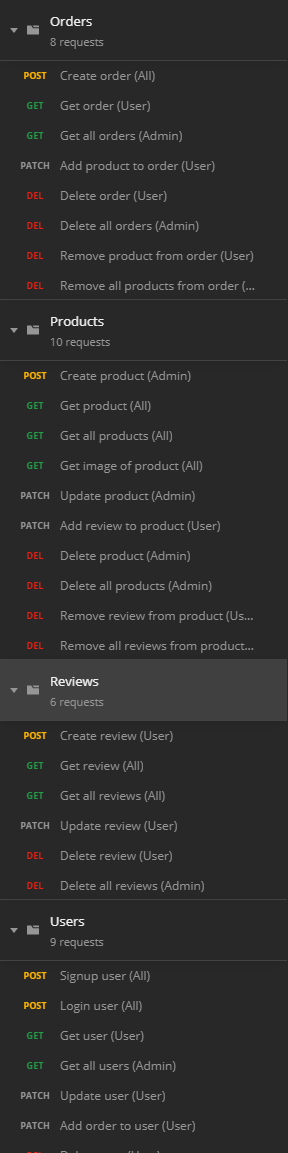
\includegraphics[width=\textwidth,height=0.6\textheight,keepaspectratio]{images/Postman_Collections.png}
 \caption{Collections in Postman}
 \label{fig:collections-postman}
\end{figure}

Abbildung \ref{fig:collections-postman} zeigt ein Teil der importieren Collections. Es gibt die Collections Orders, Products, Reviews und Users. Jede Collection enthält zugehörige Requests. Bei einem Request wird die HTTP Methode, sowie die Bennenung des Requests angezeigt. "(All)" bedeutet, dass keine Authorizierung benötigt wird. Für "(User)"  muss der Benutzer sich angemeldet haben und sein Token als Header mitversenden. Als "(Admin)" muss ein Token vorhanden sein, sowie in der Datenbank muss der Benutzer als Admin hinterlegt sein.\\
In Postman kann man einfach und Strukturiert seine Requests aufbauen. In den folgenden Abbildungen wird an dem Request "Create review (User)" die verschiedenen Hilfsmöglichkeiten gezeigt.

\begin{figure}[H]
 \centering
 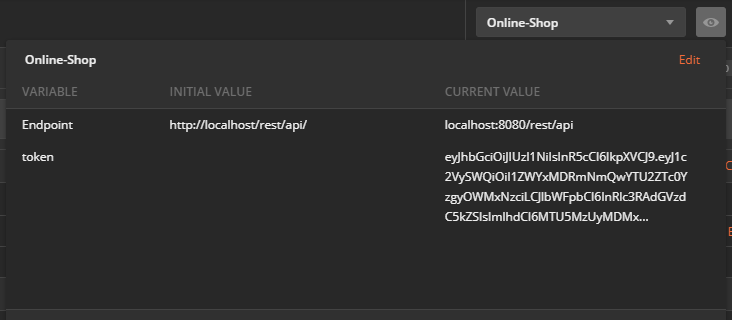
\includegraphics[width=0.8\textwidth,,keepaspectratio]{images/Postman_environment.png}
 \caption{Umgebungsvariablen in Postman}
 \label{fig:environment-postman}
\end{figure}

In Abbildung \ref{fig:environment-postman} werden die verwendeten Umgebungsvariablen gezeigt. Diese befinden sich oben rechts in Postman. Endpoint bestimmt den Basispfad der URL und token ist der Authorisierungstoken des Benutzers. Umgebungsvariablen werden mit doppelten geschweiften Klammern verwendet. Ein Beispiel dazu wäre in der Abbildung \ref{fig:authorization-postman} zu sehen.

\begin{figure}[H]
 \centering
 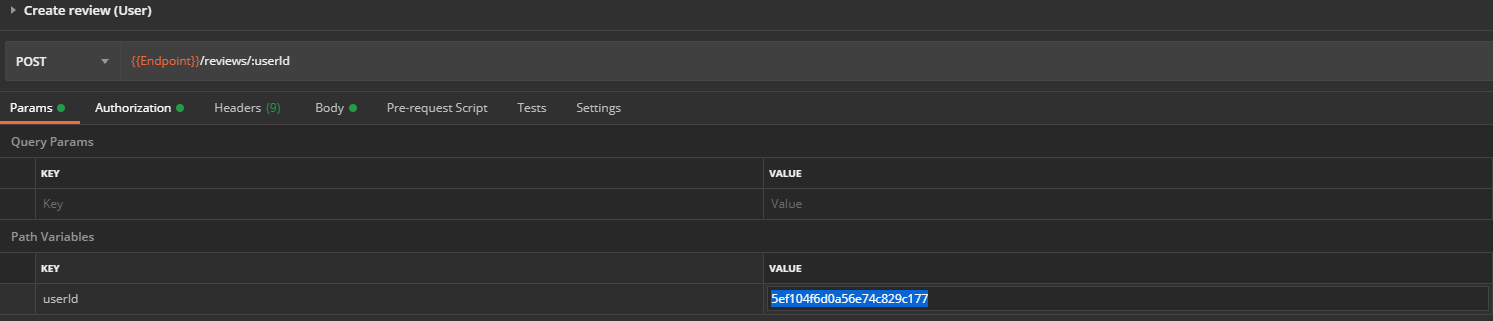
\includegraphics[width=0.9\textwidth,keepaspectratio]{images/Postman_params.png}
 \caption{Request Params in Postman}
 \label{fig:params-postman}
\end{figure}

Abbildung \ref{fig:params-postman} zeigt wie man Parameter bei einem Request eingeben kann. Dadurch muss man nicht die URL verändern, sondern kann bequem die Variablen in einer Tabelle anpassen. Parameter werden durch einen Doppelpunkt in Postman erkannt. In dieser Abbildung ist :userId ein Parameter. Dieser kann unter den Path Variables angepasst werden. Query Parameter sind Parameter die bei einem GET-Request nach dem Fragezeichen kommen.

\begin{figure}[H]
 \centering
 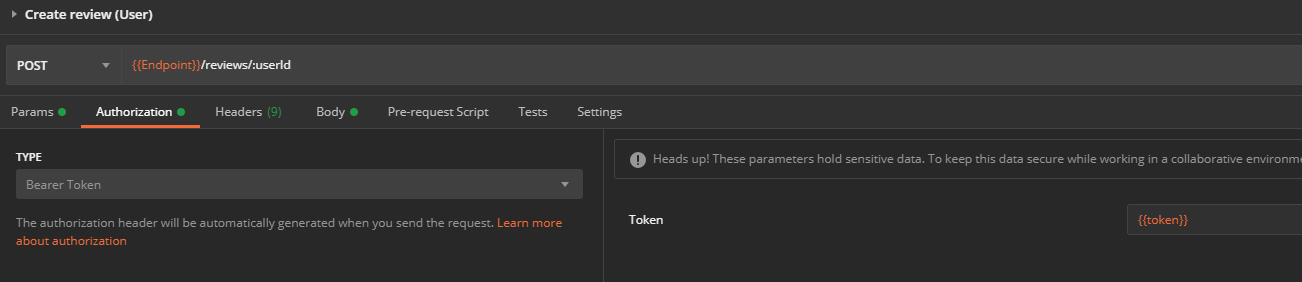
\includegraphics[width=\textwidth,height=0.6\textheight,keepaspectratio]{images/Postman_token.png}
 \caption{Request Authorization in Postman}
 \label{fig:authorization-postman}
\end{figure}

In Abbildung \ref{fig:authorization-postman} wird gezeigt wie man die Authorizierung eines Requestes festlegen kann. Im gesamten Projekt wird der Bearer Token verwendet. Diesen kann man unter TYPE festlegen. Als Token wird eine Variable definiert, dadurch muss man den Token nur einmal kopieren und als Umgebungsvariable festlegen. Den Token erhält man, sobald sich ein Benutzer anmeldet.

\begin{figure}[H]
 \centering
 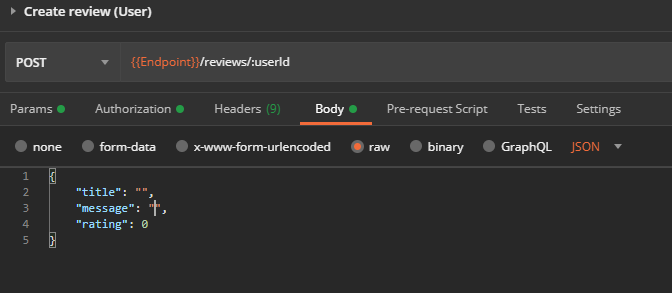
\includegraphics[width=0.75\textwidth,height=0.6\textheight,keepaspectratio]{images/Postman_body.png}
 \caption{Request Body in Postman}
 \label{fig:body-postman}
\end{figure}

Unter dem Reiter Body kann bei POST und PATCH Requests ein Inhalt mitversendet werden. Bis auf den "Create product (Admin)" Request ist der Body immer im JSON Format, siehe Abbildung \ref{fig:body-postman}.